\subsection{QuizziPedia::Back-End::App::Controllers}
\label{QuizziPedia::Back-End::App::Controllers}
\begin{figure}
	\centering
	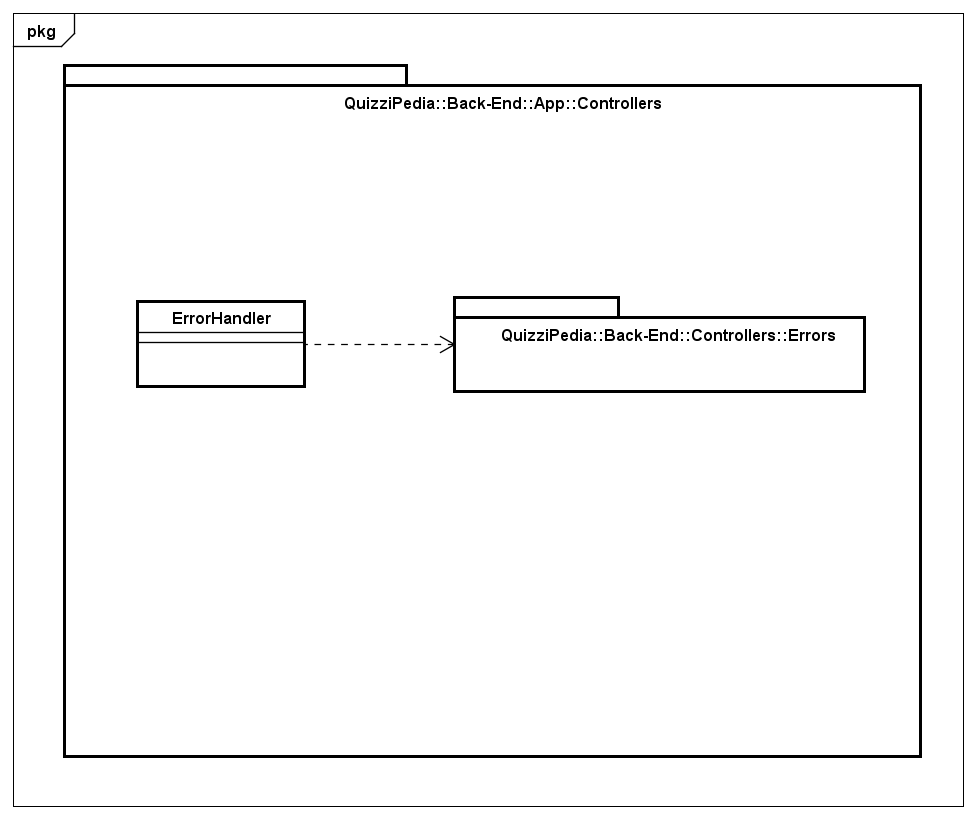
\includegraphics[scale=0.45]{UML/Package/QuizziPedia_Back-End_App_Controllers.png}
	\caption{QuizziPedia::Back-End::App::Controllers}
\end{figure}
\subsubsection{Informazioni generali}
	\begin{itemize}
		\item \textbf{Descrizione} \\
		Package contenente i controllers di Express, definisce la logica dell'applicazione.
		\item \textbf{Padre}: \texttt{App}
		\item \textbf{Interazioni con altri componenti}
			\begin{itemize}
				\item \texttt{Routers} \\
				Package contenente i router della componente back-end dell'applicazione. Contiene i file di configurazione relativi al routing delle richieste del client, ossia i routers di Express.
				\item \texttt{Views} \\
				Package contenente le views della copmonente back-end dell'applicazione.
			\end{itemize}
		\item \textbf{Package contenuti}:
			\begin{itemize}
				\item \texttt{Errors} \\
				Package contenente i controllers per la gestione degli errori specifici.
			\end{itemize}
	\end{itemize}
\subsubsection{Classi}
\paragraph{QuizziPedia::Back-End::App::Controllers::NOMECLASSE}
\begin{itemize}
	\item \textbf{Descrizione} \\
	\item \textbf{Utilizzo} \\
	\item \textbf{Relazioni con altre classi} \\
	\item \textbf{Metodi} \\
\end{itemize}